\documentclass[sigconf]{acmart}

\usepackage{booktabs} % For formal tables
\usepackage[utf8]{inputenc}
\usepackage[spanish]{babel}
\usepackage{multirow}
\usepackage{blindtext}
\usepackage{graphicx}
% The next six lines come directly from the completed rights form.
% You MUST replace them with the lines specific to your accepted work.
\copyrightyear{2017}
\acmYear{2017}
\setcopyright{rightsretained}
\acmConference{UNAM}{ENES}{CAMPUS MORELIA}


% Use the "authoryear" citation style, and make sure citations are in [square brackets].
\citestyle{acmauthoryear}
\setcitestyle{square}

% A useful command for controlling the number of authors per row.
% The default value of "authorsperrow" is 2.
%\settopmatter{authorsperrow=4}

% end of preamble.

\begin{document}


% Title. 
% If your title is long, consider \title[short title]{full title} - "short title" will be used for running heads.
\title{Death Row Information in Texas Department of Criminal Justice \\ Reglas de Asociación aplicada al listado del Departamento de Justicia de Texas}
% Authors.
\author{Karen Jaqueline Reyes Flores}
\affiliation{%
  \department{Lic.Tecnologias para la Información en Ciencias}
  \institution{UNAM, ENES CAMPUS MORELIA}}
\email{karenreyes346@gmail.com}

\author{Alejandra Guadalupe Esquivel Guillén}
\affiliation{%
  \department{Lic.Tecnologias para la Información en Ciencias}
  \institution{UNAM, ENES CAMPUS MORELIA}}
\email{alejandraeg9899@gmail.com}
% This command defines the author string for running heads.
\renewcommand{\shortauthors}{MINERIA DE DATOS}
\renewcommand{\abstractname}{Resumen}
% abstract
\begin{abstract}
En el estado de Texas el registro de armas de fuego no es requerido, aunque para la portabilidad de una, por ley se requiere una identificación emitida por el estado, esto se aplica a todos los compradores. La falta del registro de armas de fuego en el estado dificulta informar con exactitud cuántas personas poseen una. Existen 4,900 comerciantes de armas en Texas registrados.

En pleno siglo XXI existen prejuicios respecto a los delincuentes, juzgando a estos por la raza, el nivel académico logrado y los lugares de origen.

El objetivo en el presente trabajo es realizar un análisis en el cual se tratará de encontrar cierto patrón que nos lleve a determinar que no es necesario ser de tal o cual raza para cometer un delito, mostrando que los prejuicios no están del todo bien.
La idea principal a trabajar es llevar a cabo una tarea de aprendizaje denominada Reglas de Asociación, esto con la finalidad de saber cómo es que con los datos que se obtuvieron sobre una base de datos criminal del estado de Texas están relacionados.
\\Por ejemplo: Deseábamos saber si el grado de escolaridad, la raza y el lugar de origen influyen en los crimenes.

\end{abstract}

%keywords
\keywords{Algoritmo A priori, Minería de Datos, Reglas de Asociación, Discretización}

% A "teaser" figure, centered below the title and authors and above the body of the work.
\begin{teaserfigure}
  \centering
  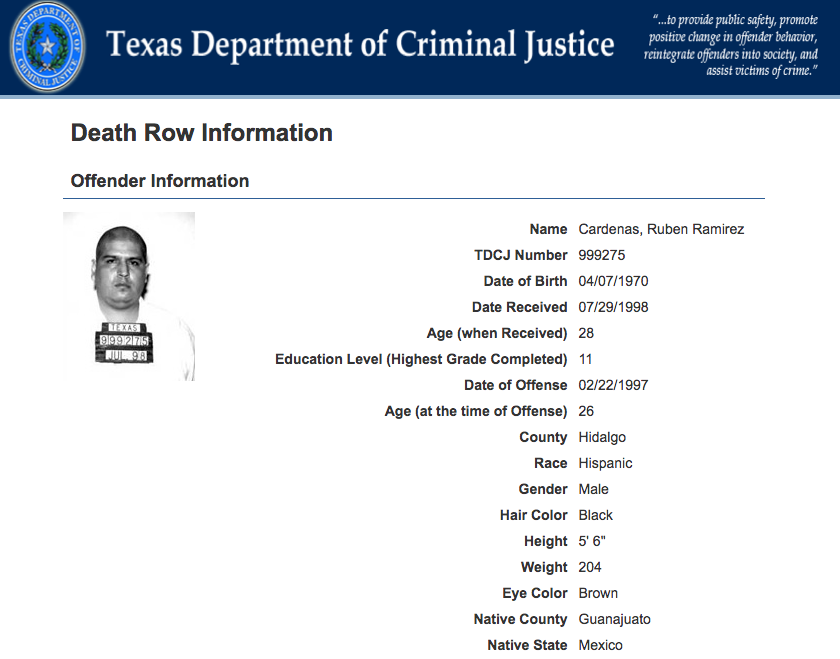
\includegraphics[width=4.0in]{C.png}
  \caption{Ficha Informativa del departamento de justicia de Texas.}
\end{teaserfigure}

% Processes all of the front-end information and starts the body of the work.
\maketitle



\section{Introducción}
En minería de datos y aprendizaje automático, las reglas de asociación se utilizan para descubrir hechos que ocurren en común dentro de un determinado conjunto de datos. El problema de minería de reglas de asociación se define como:\\
Sea $I={i_{1},i_{2},...,i_{n}}$ un conjunto de ${n}$ atributos binarios llamados items.
Sea $D={t_{1},t_{2},...,t_{m}}$ un conjunto de transacciones almacenadas en un conjunto de datos.
Cada transacción en $D$ tiene un ID (identificador) único y contiene un subconjunto de items de $I$. 
Una regla se define como una implicación de la forma: $X\Rightarrow Y$
Donde:
\begin{eqnarray*}
\begin{matrix}
X,Y\subseteq I \\
X\cap Y =\oslash
\end{matrix}
\end{eqnarray*}

Los conjuntos de items $X$ y $Y$ se denominan respectivamente "antecedente" (o parte izquierda) y "consecuente" (o parte derecha) de la regla.
La ventaja de los algoritmos de reglas de asociación sobre los algoritmos de árboles de decisión es que las asociaciones pueden existir entre cualquiera de los atributos. Un algoritmo de árbol de decisión generará reglas con una única conclusión, mientras que los algoritmos de asociación tratan de buscar muchas reglas, cada una de las cuales puede tener una conclusión diferente.
El algoritmo Apriori extrae un conjunto de reglas de los datos y destaca aquellas reglas con un mayor contenido de información.\\ Precisamente es lo que deseamos encontrar en nuestro análisis, un conjunto de reglas que nos generen información respecto a los criminales y nos den patrones comunes dentro de los asesinos registrados en la base de datos.\\Seria muy interesante poderlo aplicar para saber las tendencias que existen en los crímenes de asesinatos en Texas y así tomar medidas de precaución tal vez, en tutelares de menores o en las mismas escuelas.
\begin{figure}[ht]
  \centering
  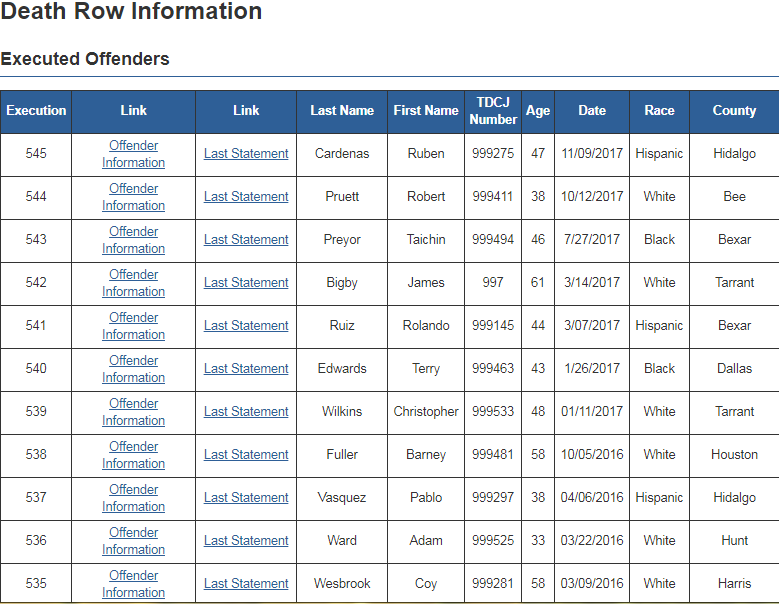
\includegraphics[width=2.5in]{d.PNG}
 % 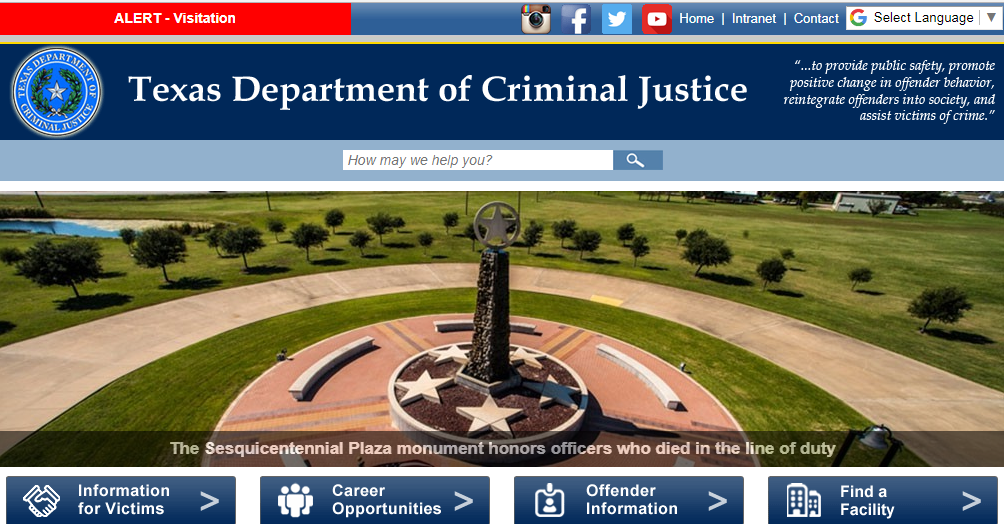
\includegraphics[width=2.5in]{C2.PNG}
  \caption{Listado de ejecuciones (13/oct/2017)}
  \label{fig:deathRow}
\end{figure}

\section{DataSet}
Del Departamento de Justicia de Texas ~\cite{DeathRow} se obtuvo un listado de las ejecuciones que se realizaron desde el 7 de Diciembre de 1982 hasta 9 de Noviembre del 2017 en el cual se incluyen las atributos descritos a continuación:

\begin{table}[ht]
\begin{center}
\scalebox{0.8}{
\begin{tabular}{|l|l|l|}
\hline
\multicolumn{1}{|c|}{Atributo} & \multicolumn{1}{c|}{Significado} & \multicolumn{1}{c|}{Tipo de Dato} \\
\hline
Execution & Número de ejecuciones & numérico \\ 
\hline
Offender Information & Información detallada & hipervínculo \\ 
\hline
Last Statement & Últimas palabras & hipervínculo \\ 
\hline
Last Name & Apellido & texto \\ 
\hline
First Name & Nombre & texto \\ 
\hline
TDCJ Number & Número de expediente & numérico \\ 
\hline
Age & Edad ejecución & numérico \\ 
\hline
Date & Fecha de ejecución & numérico \\ 
\hline
Race & Raza & texto \\ 
\hline
Country & Lugar donde se cometió el crimen & texto \\ 
\hline
\end{tabular}}
\end{center}
\caption{Listado de atributos del Departamento de Justicia}
\label{tab:dataset}
\end{table}

El hipervínculo Offender Information en el cuadro ~\ref{tab:dataset} vincula la información que se muestra en la figura ~\ref{fig:deathRow}, de la cual se decidió considerar únicamente los atributos mostrados en el cuadro ~\ref{tab:offender} debido a que estos son relevantes para nuestro estudio.


\begin{figure}[ht]
  \centering
  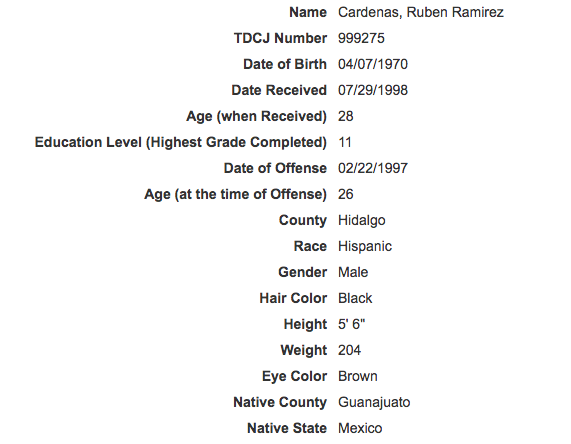
\includegraphics[width=2.5in]{datos.png}
  \caption{Atributo: Offender Information}
\end{figure}

\begin{table}[!hbt]
\begin{center}
\begin{tabular}{|l|}
\hline
Atributo\\
\hline
Education Level(Highest Grade Completed)\\
Gender\\
Native Country\\
Native State\\
\hline
\end{tabular}
\caption{Atributos seleccionados}
\label{tab:offender}
\end{center}
\end{table}


\section{Desarrollo}
Se desarrolló una herramienta que descargara los vínculos de la tabla de Information Offender los cuales venían con formato html y se convirtieron a csv, de ahí se eliminaron las columnas innecesarias y con la ayuda de open refine se editaron y eliminaron las palabras no necesarias, además se convirtieron a atributos numéricos. El proceso anterior generó 170 registros, además se encontraron 381 con formato jpg los cuales fueron procesados manualmente.
Aquellos registros cuya información no quedó completa fueron marcados como NA, finalmente sin considerar los NA se obtuvieron un total de 492 registros viables de análisis.


El DataSet contaba con 492 registros, 2 atributos continuos (Edad y Escolaridad) y 4 categóricos (Género, Condado Nativo, Raza ,Condado donde se cometió el delito). Para aplicar el algoritmo Apriori de esta investigación (se describe a continuación) se requería que el Nivel de Escolaridad fuera una variable categórica tomando los valores de Primaria en el rango de [3.. 6], Secundaria en el rango de  [7.. 9], Prepa en el rango de  [10.. 12] y Licenciatura en el rango de  [13.. 20] también la Edad se requiere que sea una variable categórica tomando valores de Veinte en el rango de [20.. 30], Treinta en el rango de [31.. 40], Cuarenta en el rango de [41.. 50], Cincuenta en el rango de [51.. 60], Sesenta en el rango de [61.. 70].


\begin{figure}[ht]
  \centering
  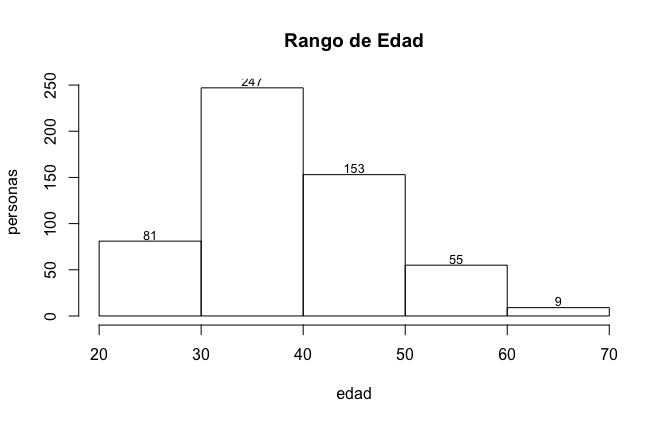
\includegraphics[width=2.5in]{Rplot.png}
  \caption{Histograma que muestra el rango de edades.}
  \label{fig:rangoEdad}
\end{figure}

\begin{figure}[ht]
  \centering
  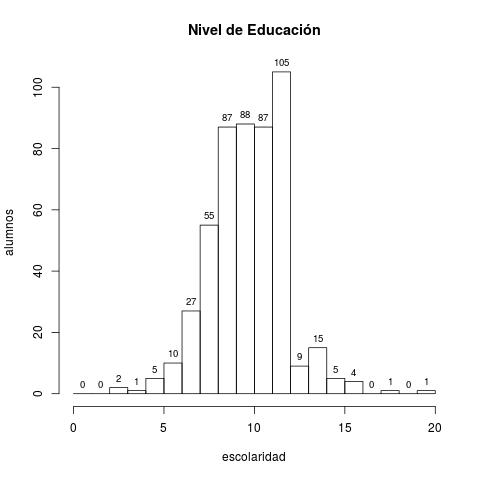
\includegraphics[width=2.5in]{escolaridad.jpg}
  \caption{Histograma que muestra el rango del nivel de  escolaridad.}
  \label{fig:rangoEscolaridad}
\end{figure}


\begin{table}[hbt]
\begin{center}
\begin{tabular}{llllll}
\toprule
educationLevel &   nativeCounty &        Age &      Race &   County \\
\midrule
         prepa &     Guanajuato &  cincuenta &  Hispanic &  Hidalgo \\
     secundaria &         Harris &   cuarenta &     White &      Bee \\
         prepa &          Bexar &   cuarenta &     Black &    Bexar \\
         prepa &         Dallas &   cuarenta &     Black &   Dallas \\
        prepa &  Harris County &  cincuenta &     White &  Tarrant \\
\bottomrule
\end{tabular}
\label{categorias}
\caption{Dataset resultante de eliminación de atributos continuos por discretos.}
\end{center}
\end{table}

\subsection{A priori} 
El algoritmo a priori~\cite{Raschka-rules} es un algoritmo utilizado en minería de datos, sobre bases de datos transaccionales, que permite encontrar de forma eficiente ``conjuntos de ítems frecuentes", los cuales sirven de base para generar reglas de asociación.

El algoritmo a priori recibe una matriz binaria y regresa los patrones frecuentes.


\section{Resultados}
El resultado del análisis fue congruente con lo que observamos en la figura \ref{fig:rangoEdad} y la figura \ref{fig:rangoEscolaridad} en donde si ordenamos por nivel de confianza y lift, lo que arroja la regla de asociación nos dicen que lo más frecuente es que el criminal tenga 30 años al momento del crimen y su grado de escolaridad sea secundaria que corresponde a un rango de entre [7.. 9 años], la segunda regla nos dice que tiene la escolaridad antes mencionada y es un hombre blanco, la tercera es que tenga la misma edad antes mencionada y sea de Harris, Texas.

\begin{table}[bt]
\scalebox{0.8}{
\begin{tabular}{lllrrrr}
\toprule
              antecedants & consequents &   support &  confidence &  lift\\
\midrule
    (treinta, secundaria) &      (Male) &  0.168699 &    1.000000 &  1.00613\\
     (White, secundaria) &      (Male) &  0.144309 &    1.000000 &  1.00613 \\
       (treinta, Harris) &      (Male) &  0.130081 &    1.000000 &  1.00613 \\
       (White, cuarenta) &      (Male) &  0.140244 &    1.000000 &  1.00613 \\
        (treinta, White) &      (Male) &  0.182927 &    1.000000 &  1.00613 \\
      (secundaria, Black) &      (Male) &  0.117886 &    1.000000 &  1.00613 \\
         (Harris, Black) &      (Male) &  0.142276 &    1.000000 &  1.00613\\
        (cuarenta, prepa) &      (Male) &  0.156504 &    1.000000 &  1.00613 \\
         (treinta, prepa) &      (Male) &  0.247967 &    0.991803 &  0.99788 \\
          (White, prepa) &      (Male) &  0.225610 &    0.990991 &  0.99707 \\
         (treinta, Black) &      (Male) &  0.186992 &    0.989130 &  0.99519 \\
          (Harris, prepa) &      (Male) &  0.146341 &    0.986111 &  0.99216 \\
          (Black, prepa) &      (Male) &  0.247967 &    0.983607 &  0.98964 \\
  (treinta, Black, prepa) &      (Male) &  0.119919 &    0.983051 &  0.98908 \\
\bottomrule
\end{tabular}}
\caption{Como se llama esta tabla}
\label{tab:resultado}
\end{table}

\begin{table}[bt]
\begin{tabular}{lllrrrr}
\toprule
  antecedants & consequents &   support &  confidence &      lift \\
\midrule
  (secundaria) &      (Male) &  0.337398 &    1.000000 &  1.006135 \\
     (treinta) &      (Male) &  0.453252 &    0.995516 &  1.001623  \\
       (White) &      (Male) &  0.441057 &    0.995392 &  1.001498 \\
     (Black) &      (Male) &  0.384146 &    0.989418 &  0.995488  \\
      (prepa) &      (Male) &  0.558943 &    0.989091 &  0.995159 \\
\bottomrule
\end{tabular}
\caption{Como se llama esta tabla}
\label{tab:resultado}
\end{table}


\subsection{Evaluación de Resultados}
Para determinar que una regla es significativa se requiere de varias medidas como \textbf{el soporte, la confianza y el lift:}\\
El 'soporte' de un conjunto de items se define como la proporción de transacciones en la base de datos que contiene dicho conjunto de items:
\begin{equation} \label{eq:solve}
Soporte(X)=\frac{|X|}{|D|}
\end{equation}
La 'confianza' de una regla puede interpretarse como un estimador de ${\displaystyle P(Y|X)} {\displaystyle P(Y|X)}$, la probabilidad de encontrar la parte derecha de una regla condicionada a que se encuentre también la parte izquierda.:
\begin{equation} \label{eq:solve}
{\displaystyle \mathrm {conf} (X\Rightarrow Y)={\frac {\mathrm {sop} (X\cup Y)}{\mathrm {sop} (X)}}={\frac {\left|X\cup Y\right\vert }{\left|X\right\vert }}}
\end{equation}
El 'lift' expresa cuál es la proporción del soporte observado de un conjunto de productos respecto del soporte teórico de ese conjunto dado el supuesto de independencia. 




\section{Conclusiones}
A contrario de lo que se piensa comúnmente en los estados unidos, las reglas de asociación nos demostraron que es más común que los criminales que fueron asesinados mediante la pena de muerte, son personas de raza blanca con un $44\%$ en nivel de soporte en contradicción de la raza negra con un $38\%$ de soporte. Y respecto al grado de escolaridad, los criminales con mayor nivel de soporte fueron los que estudiaron la preparatoria (9-12 años) con un nivel de $55\%$ y los que estudiaron la secundaria fue de $33\%$.\\ Creemos que sería de gran ayuda este análisis de patrones o reglas frecuentes para localizar ciertos focos rojos en los tutelares para menores de Texas e intentar prevenir más penas de muerte en este estado, y reducir la cantidad de crímenes que en estos últimos años ha ido en incremento en dicha zona.\\




\bibliography{aaatemplate}{}
\bibliographystyle{ACM-Reference-Format}

 
\end{document}